\section{Introduction}
We test the utility of the $K$-means algorithm in assigning grades
as compared to estimating the grades using the standard normal 
distribution.

We consider the scores of $N = 94$ students who have taken a course in the 
Indian Institute of Technology, Hyderabad (IITH) as our dataset.

\section{Fitting a Gaussian Curve}
Since $N$ is not very large, given the scores of each student 
$x_i,\ 1 \le i \le N$, we can compute the population mean and population 
variance as

\begin{align}
    \mu &= \mean{x} \\
    \sigma^2 &= \mean{\brak{x-\mu}^2}
    \label{eq:pop-param}
\end{align}

We assume that the scores $x \sim N\brak{\mu,\sigma^2}$. Thus, we compute the
$Z$-scores as
\begin{align}
    Z = \frac{x-\mu}{\sigma}
\end{align}

The grades are assigned as per Table \ref{tab:grade-scheme}.
\begin{table}[!ht]
    \centering
    %%%%%%%%%%%%%%%%%%%%%%%%%%%%%%%%%%%%%%%%%%%%%%%%%%%%%%%%%%%%%%%%%%%%%%
%%                                                                  %%
%%  This is the header of a LaTeX2e file exported from Gnumeric.    %%
%%                                                                  %%
%%  This file can be compiled as it stands or included in another   %%
%%  LaTeX document. The table is based on the longtable package so  %%
%%  the longtable options (headers, footers...) can be set in the   %%
%%  preamble section below (see PRAMBLE).                           %%
%%                                                                  %%
%%  To include the file in another, the following two lines must be %%
%%  in the including file:                                          %%
%%        \def\inputGnumericTable{}                                 %%
%%  at the beginning of the file and:                               %%
%%        \input{name-of-this-file.tex}                             %%
%%  where the table is to be placed. Note also that the including   %%
%%  file must use the following packages for the table to be        %%
%%  rendered correctly:                                             %%
%%    \usepackage[latin1]{inputenc}                                 %%
%%    \usepackage{color}                                            %%
%%    \usepackage{array}                                            %%
%%    \usepackage{longtable}                                        %%
%%    \usepackage{calc}                                             %%
%%    \usepackage{multirow}                                         %%
%%    \usepackage{hhline}                                           %%
%%    \usepackage{ifthen}                                           %%
%%  optionally (for landscape tables embedded in another document): %%
%%    \usepackage{lscape}                                           %%
%%                                                                  %%
%%%%%%%%%%%%%%%%%%%%%%%%%%%%%%%%%%%%%%%%%%%%%%%%%%%%%%%%%%%%%%%%%%%%%%



%%  This section checks if we are begin input into another file or  %%
%%  the file will be compiled alone. First use a macro taken from   %%
%%  the TeXbook ex 7.7 (suggestion of Han-Wen Nienhuys).            %%
\def\ifundefined#1{\expandafter\ifx\csname#1\endcsname\relax}


%%  Check for the \def token for inputed files. If it is not        %%
%%  defined, the file will be processed as a standalone and the     %%
%%  preamble will be used.                                          %%
\ifundefined{inputGnumericTable}

%%  We must be able to close or not the document at the end.        %%
	\def\gnumericTableEnd{\end{document}}


%%%%%%%%%%%%%%%%%%%%%%%%%%%%%%%%%%%%%%%%%%%%%%%%%%%%%%%%%%%%%%%%%%%%%%
%%                                                                  %%
%%  This is the PREAMBLE. Change these values to get the right      %%
%%  paper size and other niceties.                                  %%
%%                                                                  %%
%%%%%%%%%%%%%%%%%%%%%%%%%%%%%%%%%%%%%%%%%%%%%%%%%%%%%%%%%%%%%%%%%%%%%%

	\documentclass[12pt%
			  %,landscape%
                    ]{report}
       \usepackage[latin1]{inputenc}
       \usepackage{fullpage}
       \usepackage{color}
       \usepackage{array}
       \usepackage{longtable}
       \usepackage{calc}
       \usepackage{multirow}
       \usepackage{hhline}
       \usepackage{ifthen}

	\begin{document}


%%  End of the preamble for the standalone. The next section is for %%
%%  documents which are included into other LaTeX2e files.          %%
\else

%%  We are not a stand alone document. For a regular table, we will %%
%%  have no preamble and only define the closing to mean nothing.   %%
    \def\gnumericTableEnd{}

%%  If we want landscape mode in an embedded document, comment out  %%
%%  the line above and uncomment the two below. The table will      %%
%%  begin on a new page and run in landscape mode.                  %%
%       \def\gnumericTableEnd{\end{landscape}}
%       \begin{landscape}


%%  End of the else clause for this file being \input.              %%
\fi

%%%%%%%%%%%%%%%%%%%%%%%%%%%%%%%%%%%%%%%%%%%%%%%%%%%%%%%%%%%%%%%%%%%%%%
%%                                                                  %%
%%  The rest is the gnumeric table, except for the closing          %%
%%  statement. Changes below will alter the table's appearance.     %%
%%                                                                  %%
%%%%%%%%%%%%%%%%%%%%%%%%%%%%%%%%%%%%%%%%%%%%%%%%%%%%%%%%%%%%%%%%%%%%%%

\providecommand{\gnumericmathit}[1]{#1} 
%%  Uncomment the next line if you would like your numbers to be in %%
%%  italics if they are italizised in the gnumeric table.           %%
%\renewcommand{\gnumericmathit}[1]{\mathit{#1}}
\providecommand{\gnumericPB}[1]%
{\let\gnumericTemp=\\#1\let\\=\gnumericTemp\hspace{0pt}}
 \ifundefined{gnumericTableWidthDefined}
        \newlength{\gnumericTableWidth}
        \newlength{\gnumericTableWidthComplete}
        \newlength{\gnumericMultiRowLength}
        \global\def\gnumericTableWidthDefined{}
 \fi
%% The following setting protects this code from babel shorthands.  %%
 \ifthenelse{\isundefined{\languageshorthands}}{}{\languageshorthands{english}}
%%  The default table format retains the relative column widths of  %%
%%  gnumeric. They can easily be changed to c, r or l. In that case %%
%%  you may want to comment out the next line and uncomment the one %%
%%  thereafter                                                      %%
\providecommand\gnumbox{\makebox[0pt]}
%%\providecommand\gnumbox[1][]{\makebox}

%% to adjust positions in multirow situations                       %%
\setlength{\bigstrutjot}{\jot}
\setlength{\extrarowheight}{\doublerulesep}

%%  The \setlongtables command keeps column widths the same across  %%
%%  pages. Simply comment out next line for varying column widths.  %%
\setlongtables

\setlength\gnumericTableWidth{%
	53pt+%
	53pt+%
0pt}
\def\gumericNumCols{2}
\setlength\gnumericTableWidthComplete{\gnumericTableWidth+%
         \tabcolsep*\gumericNumCols*2+\arrayrulewidth*\gumericNumCols}
\ifthenelse{\lengthtest{\gnumericTableWidthComplete > \linewidth}}%
         {\def\gnumericScale{\ratio{\linewidth-%
                        \tabcolsep*\gumericNumCols*2-%
                        \arrayrulewidth*\gumericNumCols}%
{\gnumericTableWidth}}}%
{\def\gnumericScale{1}}

%%%%%%%%%%%%%%%%%%%%%%%%%%%%%%%%%%%%%%%%%%%%%%%%%%%%%%%%%%%%%%%%%%%%%%
%%                                                                  %%
%% The following are the widths of the various columns. We are      %%
%% defining them here because then they are easier to change.       %%
%% Depending on the cell formats we may use them more than once.    %%
%%                                                                  %%
%%%%%%%%%%%%%%%%%%%%%%%%%%%%%%%%%%%%%%%%%%%%%%%%%%%%%%%%%%%%%%%%%%%%%%

\ifthenelse{\isundefined{\gnumericColA}}{\newlength{\gnumericColA}}{}\settowidth{\gnumericColA}{\begin{tabular}{@{}p{53pt*\gnumericScale}@{}}x\end{tabular}}
\ifthenelse{\isundefined{\gnumericColB}}{\newlength{\gnumericColB}}{}\settowidth{\gnumericColB}{\begin{tabular}{@{}p{53pt*\gnumericScale}@{}}x\end{tabular}}

\begin{tabular}[c]{%
	b{\gnumericColA}%
	b{\gnumericColB}%
	}

%%%%%%%%%%%%%%%%%%%%%%%%%%%%%%%%%%%%%%%%%%%%%%%%%%%%%%%%%%%%%%%%%%%%%%
%%  The longtable options. (Caption, headers... see Goosens, p.124) %%
%	\caption{The Table Caption.}             \\	%
% \hline	% Across the top of the table.
%%  The rest of these options are table rows which are placed on    %%
%%  the first, last or every page. Use \multicolumn if you want.    %%

%%  Header for the first page.                                      %%
%	\multicolumn{2}{c}{The First Header} \\ \hline 
%	\multicolumn{1}{c}{colTag}	%Column 1
%	&\multicolumn{1}{c}{colTag}	\\ \hline %Last column
%	\endfirsthead

%%  The running header definition.                                  %%
%	\hline
%	\multicolumn{2}{l}{\ldots\small\slshape continued} \\ \hline
%	\multicolumn{1}{c}{colTag}	%Column 1
%	&\multicolumn{1}{c}{colTag}	\\ \hline %Last column
%	\endhead

%%  The running footer definition.                                  %%
%	\hline
%	\multicolumn{2}{r}{\small\slshape continued\ldots} \\
%	\endfoot

%%  The ending footer definition.                                   %%
%	\multicolumn{2}{c}{That's all folks} \\ \hline 
%	\endlastfoot
%%%%%%%%%%%%%%%%%%%%%%%%%%%%%%%%%%%%%%%%%%%%%%%%%%%%%%%%%%%%%%%%%%%%%%

\hhline{|-|-}
	 \multicolumn{1}{|p{\gnumericColA}|}%
	{\gnumericPB{\raggedright}\gnumbox[l]{\textbf{Interval}}}
	&\multicolumn{1}{p{\gnumericColB}|}%
	{\gnumericPB{\raggedright}\gnumbox[l]{\textbf{Grade}}}
\\
\hhline{|--|}
	 \multicolumn{1}{|p{\gnumericColA}|}%
	{\gnumericPB{\raggedright}\gnumbox[l]{($-\infty$, -3]}}
	&\multicolumn{1}{p{\gnumericColB}|}%
	{\gnumericPB{\raggedright}\gnumbox[l]{F}}
\\
\hhline{|--|}
	 \multicolumn{1}{|p{\gnumericColA}|}%
	{\gnumericPB{\raggedright}\gnumbox[l]{(-3, -2]}}
	&\multicolumn{1}{p{\gnumericColB}|}%
	{\gnumericPB{\raggedright}\gnumbox[l]{D}}
\\
\hhline{|--|}
	 \multicolumn{1}{|p{\gnumericColA}|}%
	{\gnumericPB{\raggedright}\gnumbox[l]{(-2, 1]}}
	&\multicolumn{1}{p{\gnumericColB}|}%
	{\gnumericPB{\raggedright}\gnumbox[l]{C}}
\\
\hhline{|--|}
	 \multicolumn{1}{|p{\gnumericColA}|}%
	{\gnumericPB{\raggedright}\gnumbox[l]{(-1, 0]}}
	&\multicolumn{1}{p{\gnumericColB}|}%
	{\gnumericPB{\raggedright}\gnumbox[l]{B-}}
\\
\hhline{|--|}
	 \multicolumn{1}{|p{\gnumericColA}|}%
	{\gnumericPB{\raggedright}\gnumbox[l]{(0, 1]}}
	&\multicolumn{1}{p{\gnumericColB}|}%
	{\gnumericPB{\raggedright}\gnumbox[l]{B}}
\\
\hhline{|--|}
	 \multicolumn{1}{|p{\gnumericColA}|}%
	{\gnumericPB{\raggedright}\gnumbox[l]{(1, 2]}}
	&\multicolumn{1}{p{\gnumericColB}|}%
	{\gnumericPB{\raggedright}\gnumbox[l]{A-}}
\\
\hhline{|--|}
	 \multicolumn{1}{|p{\gnumericColA}|}%
	{\gnumericPB{\raggedright}\gnumbox[l]{(2, 3]}}
	&\multicolumn{1}{p{\gnumericColB}|}%
	{\gnumericPB{\raggedright}\gnumbox[l]{A}}
\\
\hhline{|--|}
	 \multicolumn{1}{|p{\gnumericColA}|}%
	{\gnumericPB{\raggedright}\gnumbox[l]{(3,$\infty$)}}
	&\multicolumn{1}{p{\gnumericColB}|}%
	{\gnumericPB{\raggedright}\gnumbox[l]{A+}}
\\
\hhline{|-|-|}
\end{tabular}

\ifthenelse{\isundefined{\languageshorthands}}{}{\languageshorthands{\languagename}}
\gnumericTableEnd

    \caption{Grading Scheme.}
    \label{tab:grade-scheme}
\end{table}

The Python code \texttt{codes/grades\_norm.py} takes the given input 
population dataset \texttt{marks.xlsx} and assigns grades appropriately. 
The grades are output to \texttt{grades.xlsx}.

\section{K-Means Clustering}
$K$-Means clustering is an unsupervised classification model, which attempts to 
cluster unlabeled data in order to gain more structure from it. 

We frame this requirement as an optimization problem. For a set of data points 
$\cbrak{\vec{x}_i}_{i=1}^N$ and means $\cbrak{\vec{\mu}_i}_{i=1}^K$, we define
for $1 \le n \le N,\ 1 \le k \le K$,
\begin{align}
    r_{nk} \triangleq
    \begin{cases}
        1 & \argmin_{j}\norm{\vec{x}_n-\vec{\mu}_j} = k \\
        0 & \textrm{otherwise}
    \end{cases}
    \label{eq:rnk-def}
\end{align}
Thus, we need to find points $\vec{\mu}_k$ minimizing the cost function
\begin{align}
    J \triangleq \sum_{n=1}^N\sum_{k=1}^Kr_{nk}\norm{\vec{x}_n-\vec{\mu}_k}^2
    \label{eq:cost}
\end{align}
Clearly, \eqref{eq:cost} is a quadratic function of $\vec{\mu}_k$.
Differentiating with respect to $\vec{\mu}_k$ and setting the derivative
to zero, we get
\begin{align}
    \sum_{n=1}^N2\vec{\mu}_kr_{nk}\brak{\vec{x}_n-\vec{\mu}_k} = 0 \\
    \implies \vec{{\mu_k}} = \frac{\sum_{n=1}^Nr_{nk}\vec{x}_n}{\sum_{n=1}^Nr_{nk}} = \frac{\vec{Xr}_k}{\vec{1}^\top\vec{r}_k}
    \label{eq:M-step}
\end{align}
where
\begin{align}
    \vec{X} &\triangleq \myvec{\vec{x}_1&\vec{x}_2&\ldots&\vec{x}_n} \\
    \vec{r}_k &\triangleq \myvec{r_{1k}&r_{2k}&\ldots&r_{nk}}^\top \\
    \vec{1} &\triangleq \myvec{1&1&\ldots&1}^\top
    \label{eq:M-defs}
\end{align}
From \eqref{eq:M-step}, we see that the optimum is attained when $\vec{\mu}_k$ 
is set to the expectation of the $\vec{x}_n$ with respect to $r_{nk}$.

Thus, the $K$-means algorithm is essentially an \textit{EM algorithm}, where 
each iteration consists of two steps.
\begin{enumerate}
    \item \textit{E Step}: Calculate the $K$-expected values
    \begin{align}
        \tilde{\vec{\mu}_k} \triangleq \frac{\sum_{n=1}^Nr_{nk}\vec{x}_n}{\sum_{n=1}^Nr_{nk}}
        \label{eq:E-step}
    \end{align}
    for $1 \le k \le K$.
    \item \textit{M Step}: Assign $\vec{\mu}_k \leftarrow \tilde{\vec{\mu}_k}$
    for $1 \le k \le K$.
\end{enumerate}

\section{Results}
The grade distribution using each method is shown in Fig. \ref{fig:gauss-dist}
and Fig. \ref{fig:kmeans-dist}.
\begin{figure}[!ht]
    \centering
    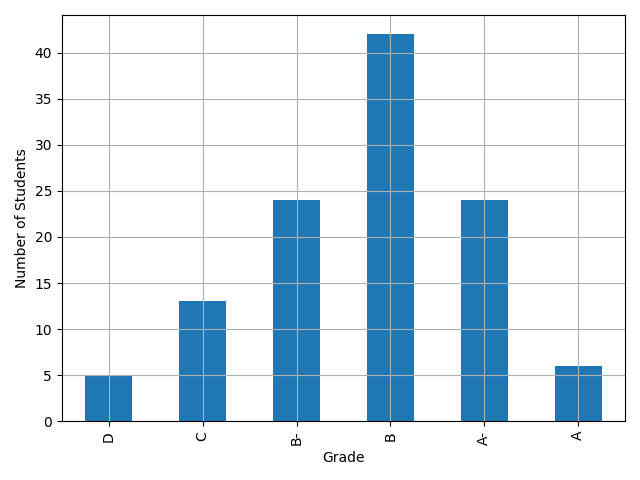
\includegraphics[width=\columnwidth]{grading/figs/grades_gauss.png}
    \caption{Grade distribution using a Gaussian curve.}
    \label{fig:gauss-dist}
\end{figure}
\begin{figure}[!ht]
    \centering
    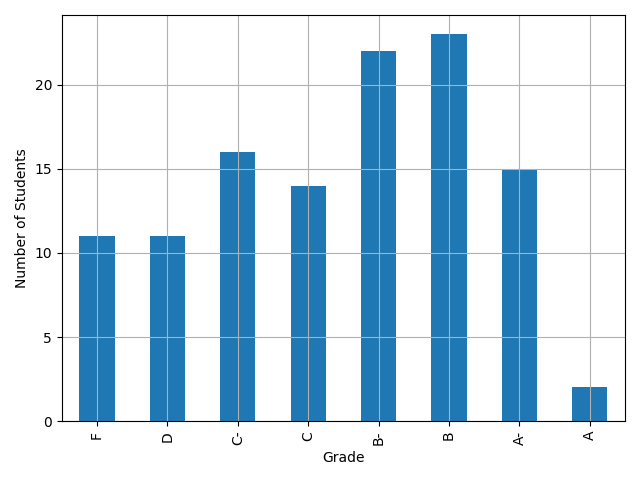
\includegraphics[width=\columnwidth]{grading/figs/grades_kmeans.png}
    \caption{Grade distribution using the $K$-means algorithm.}
    \label{fig:kmeans-dist}
\end{figure}
Based on the results, we can make the following observations:
\begin{enumerate}
    \item Grading using the Gaussian distribution would lead to many students
    failing the course, while this is not the case using the $K$-means
    algorithm.
    \item Using the Gaussian distribution is quite unfair, since there could
    be students with quite similar marks but with a difference in grade, just
    because they lie on either side of a predefined boundary.
    \item The $K$-means algorithm allows for better decision boundaries,
    depending on how skewed the performance of the students is, accordingly
    to the difficulty of the course.
    \item Unlike the Gaussian distribution, the $K$-means algorithm can be
    used for a fairer assignment of the grades, no matter how skewed the 
    performance of students in a course is.
\end{enumerate}
